\section{Results}\label{sec:METHODRESULTS}

%% here we will discuss results of our work. Consider and compare quality metrics, show interesting finding. E.g.g

In this section we will present results of both classification approaches, analyzing time complexity, memory consumption and classification accuracy.

\subsection{Discrete case}

Discrete case algorithm is a pure improvement of NSW and HNSW data structures. We run two sets of experiments. First set is based on our own implementation paper-based \cite{nsw} of NSW data structure. We added algorithm ~\ref{alg:the_alg} to \texttt{modules/nsw/nsw\_classifier.py} class. This implementation shows slight accuracy lack compared to 1-NN baseline classification, but also expose 1.5x speedup regardless of data dimensionality. See table~\ref{tab:nsw} for details.

\begin{table}
\caption{Time and accuracy performance of 1-NN and path casting classifiers}
\label{tab:nsw}
\centering
\begin{tabular}{ | p{20mm} | p{5mm} | p{10mm} | p{10mm} | p{10mm} | }
\hline
    \textbf{Test}
  & \textbf{dim.}
  & \textbf{path avg faster} 
  & \textbf{NSW 1-NN accuracy}
  & \textbf{NSW path accuracy} \\
 \hline
 Synthetic 2K & 2 & 1.33 & 97.42\% & 97.22\% \\ \hline
 Synthetic 5K & 2 & 1.46 & 99.25\% & 97.50\% \\ \hline
 Synthetic 3K & 4 & 1.62 & 92.70\% & 91.35\% \\ \hline
 Synthetic 3K & 16 & 2.73 & 53.50\% & 56.70\% \\ \hline
 Synthetic 3K & 256 & 1.43 & 54.00\% & 51.40\% \\ \hline
 handwritten (10 classes) \cite{mnist} & 64 & 1.46 & \textbf{99.44\%} & 98.33\% \\ \hline
 100 leaves (margin) \cite{100leaves} & 64 & 1.14 & 58.75\% & \textbf{71.25\%} \\ \hline
 Signs 10K \cite{signsdataset} & 256 & 1.93 & 18.00 & \textbf{37.50\%} \\ \hline
\end{tabular}
\end{table}

Of course, naive python implementation has no practical profit. Thus, for a second set of experiments we implemented a patch to C++ GitHub repository\footnote{\texttt{hnswlib repo} codebase: \url{https://github.com/nmslib/hnswlib}.}, created by authors of original HNSW paper \cite{hnsw}.
Luckily, for this implementation we got surprisingly bigger time improvement. We cannot state, that implementation of data structure in repository is exactly the same as described in paper, as repository was active development phase in 2017-2020 years. Thus our improvement cannot be considered as exact implementation of proposed algorithm. You can examine insignificant difference between proposed algorithm and its implementation in a library in our repository in \texttt{nhswlib/hnswalg.h} file history.
Our implementation adds to original implementation a dictionary, representing classes of objects. In practice this means $4*|V|$ bytes memory overhead.
Time and accuracy comparison are presented in table~\ref{tab:hnswlib}.

\begin{table}
\caption{Synthetic (100K items) speed test and accuracy for hnswlib}
\label{tab:hnswlib}
\centering
\begin{tabular}{ | p{5mm} | p{7mm} | p{7mm} | p{7mm} | p{7mm} | p{7mm} | p{7mm} | }
\hline
  {\rotatebox{90}{\textbf{Dimensions}}}
  & {\rotatebox{90}{\textbf{NSW path acc., \%}}}
  & {\rotatebox{90}{\textbf{NSW path time, ms}}}
  & {\rotatebox{90}{\textbf{HNSW path acc., \%}}}
  & {\rotatebox{90}{\textbf{HNSW path time, ms}}}
  & {\rotatebox{90}{\textbf{HNSW 1-NN acc., \%}}}
  & {\rotatebox{90}{\textbf{HNSW 1-NN time, ms}}} \\
 \hline
 2 & 11.99 & 98.26 & \textbf{3.76} & 99.62 & 31.36 & 99.94 \\ \hline
 4 & 9.05 & 95.24 & \textbf{4.41} & 96.32 & 72.36 & 98.58 \\ \hline
 8 & 10.01 & 84.86 & \textbf{6.25} & 85.18 & 80.87 & 91.52 \\ \hline
 10 & \textbf{8.55} & 80.3 & \textbf{8.07} & 80.84 & 107.58 & 88.1 \\ \hline
 16 & \textbf{13.95} & 74.78 & \textbf{12.04} & 74.38 & 189.98 & 82.8 \\ \hline
\end{tabular}
\end{table}

\subsection{Continuous case}

Continuous case is a separate method, which uses NSW graph construction phase, but holding a separate data structure. In this paper we prepared only Python implementation of this method, thus we cannot compete with other methods in speed right now. We discuss further steps in section~\ref{sec:DISCUSSION}. Here we focus on practical memory consumption and classification accuracy.

Our method is based on saving graph cut edges only. Thus, we need to have a good estimation for cut size. We know, that by construction and recommendations of authors, graph will have $\mathcal{O}(|V|*D)$ edges at all. Higher dimensions tend to have more items laying at the border of the class. Our studies for a synthetic data showed, that graph cut size grow together with graph degree, which is by recommendations of original paper linearly depend on both dataset size and data dimensionality. See figure~\ref{fig:nswcutsize} for details.

\begin{figure}
    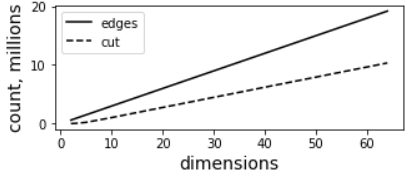
\includegraphics[width=3.3in]{paper/images/02_cutsize.png}
    \caption{Properties of NSW graph for 2-class dataset of 100K items with balanced classes and uniformly distributed features.}
    \label{fig:nswcutsize}
\end{figure}

Thus we used hyperparameter $cutsize$ which subsamples the shortest edges from the cut. Thus, for our model we have the following complete list of hyperparameters:
\begin{itemize}
    \item $cutsize$ -- cut subset size used to approximate gradient function;
    \item $R$ -- varies $\epsilon$-neighbourhood in approximation algorithm;
    \item $k$ -- number of support vectors used for voting;
    \item $N$ -- number of steps in discrete integration;
    \item $small$ -- defines zero level of integration;
\end{itemize}


We performed two types of tests for continuous case. Firstly, we created a synthetic 2-dimensional dataset with a smooth class boundary and 3\% of misclassified items in a training set. This set of tests is created to, firstly, validate the hypothesis, that a proposed classifier works, and secondly, to understand how hyperparameters influence classification accuracy.




% With growth of vector dimensions share of edges falling into NSW graph cut is increasing and tend to reach 0.5.

% Number of edges linearly growing to number of nodes. Thus, cut is linearly growing to nodes.